\documentclass[10pt,a4paper]{article}
\usepackage[utf8]{inputenc}
\usepackage[T1]{fontenc}
\usepackage[margin=0.43in]{geometry}
\usepackage{enumitem}
\usepackage{hyperref}
\usepackage{titlesec}
\usepackage{graphicx}
\usepackage{tabularx}
\usepackage{xcolor}
\usepackage{charter}

\definecolor{ink}{HTML}{15191C}
\definecolor{cobalt}{HTML}{2349D8}
\hypersetup{colorlinks=true,urlcolor=cobalt,linkcolor=cobalt}
\titleformat{\section}{\large\bfseries\uppercase\color{ink}}{}{0em}{}[\titlerule]
\titlespacing{\section}{0pt}{6pt}{3pt}
\setlist[itemize]{noitemsep,topsep=1pt,leftmargin=1.25em}
\pagestyle{empty}
\setlength{\parindent}{0pt}

\begin{document}

\begin{minipage}[t]{0.73\textwidth}
    {\huge\bfseries Sheng Lu (Lucas Lu)}\\[-1pt]
    \textbf{B.Eng. Candidate in Industrial Engineering | Class of 2029}\\[3pt]
    Email: \href{mailto:12511133@mail.sustech.edu.cn}{12511133@mail.sustech.edu.cn} \textbar\ Phone: (+86) 157-2864-3180\\
    Website: \href{https://lucas12511133.github.io}{lucas12511133.github.io}\\
    Location: Zhicheng College, Southern University of Science and Technology, Shenzhen, China
\end{minipage}
\begin{minipage}[t]{0.20\textwidth}
    \raggedleft
    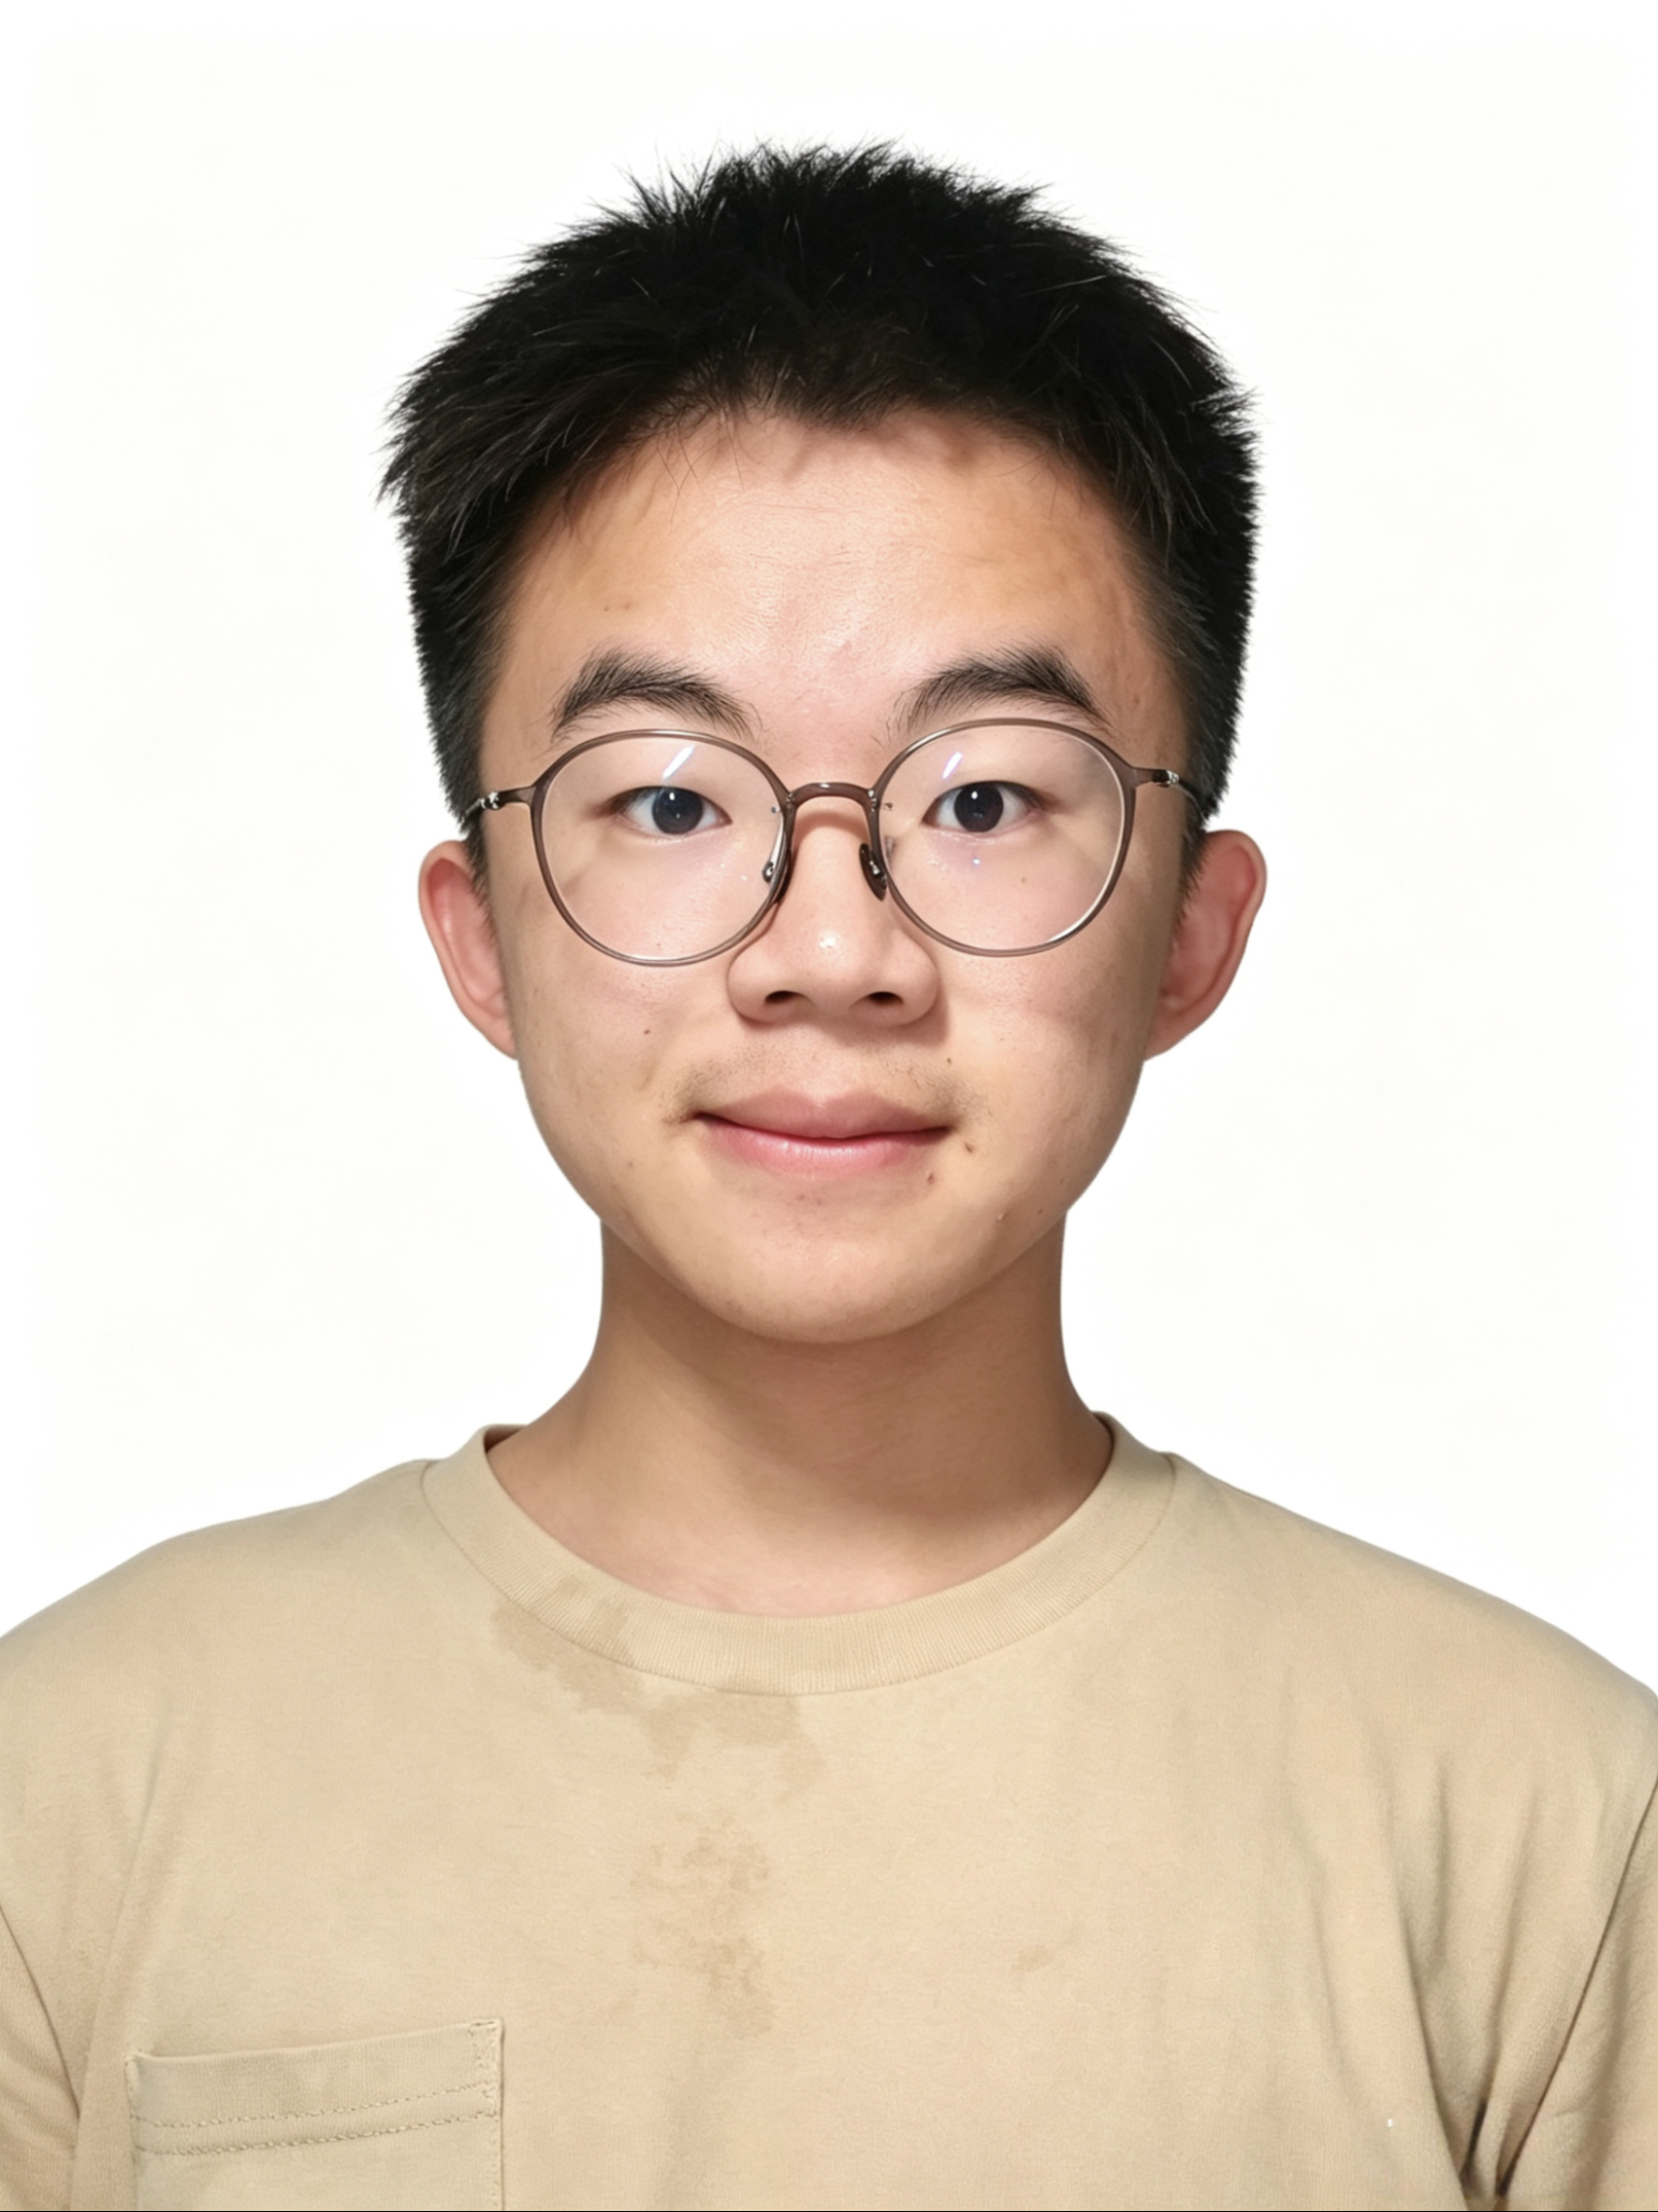
\includegraphics[width=2.35cm,height=3.05cm,keepaspectratio]{photo.png}
\end{minipage}

\vspace{3pt}

\section{Research Interests \& Mentorship}
\begin{itemize}
    \item \textbf{Interests:} Operations Research \& Optimization; Emergency Response \& Logistics; Machine Learning \& Data Science; Mathematical Modeling.
    \item \textbf{Academic Mentor:} \textbf{Professor Yu Wang}, Department of Industrial Engineering, SUSTech.
\end{itemize}

\section{Education}
\textbf{Southern University of Science and Technology (SUSTech)} \hfill Aug. 2025 -- Present\\
\textit{B.Eng. in Industrial Engineering, Zhicheng College} \hfill Shenzhen, China
\begin{itemize}
    \item \textbf{GPA: 3.91 / 4.0} \textbar\ \textbf{Ranking: 1 / 11}.
    \item \textbf{Selected Coursework:} Mathematical Analysis I--II (93, 96), Ordinary Differential Equations B (98), Foundation of Probability Theory (94), Linear Algebra (89), Introduction to C Programming (96), College Physics II (90).
\end{itemize}
\section{Selected Research \& Projects}
\textbf{EMS Station Location Optimization} \hfill 2026 -- Present\\
\textit{Project Lead | 120 EMS Station Location Optimization}
\begin{itemize}
    \item Leading a 6-member team to optimize emergency medical service station placement across Shenzhen. Partitioned the city into 5,279 500m$\times$500m grids and developed an XGBoost ETA model using 620K+ dispatch records and 360K Tencent Maps samples (MAE = 1.64 min, R$^2$ = 0.863); achieved 90\% coverage within 10 minutes.
    \item Finalist, 8th China University Mechanical Engineering Innovation \& Creativity Competition (2026). Tools: Python, OSMnx, XGBoost.
\end{itemize}
\textbf{AED Deployment at Gulongzhong} \hfill 2026 -- Present\\
\textit{Project Participant | AED Deployment at Gulongzhong}
\begin{itemize}
    \item Comparing static AED placement with a dynamic human--vehicle--drone coordinated scheme using road-network analysis; exploring sustainable operation through insurance partnership models.
\end{itemize}
\textbf{Meal Optimization WeChat Mini Program} \hfill 2026\\
\textit{Project Developer | Personalized Meal Recommendation}
\begin{itemize}
    \item Developed a WeChat mini program for personalized meal recommendations from user profiles and dietary preferences, using Taro + React + TypeScript with Tencent Cloud Functions and an optimization solver. Supported meat/vegetable/staple structure configuration, taste matching, nutrition constraints, and set-meal recommendations.
    \item Implemented upper/lower bounds for calories, protein, carbohydrates, and fats; hard-excluded disliked ingredients, dish-level replacement, infeasibility fallbacks, and carbohydrate-overage alerts with adjustment suggestions. Improved stability and UX through legacy solver compatibility, exception fallback, and frontend feedback.
\end{itemize}

\section{Selected Honors \& Awards}
\begin{itemize}
    \item \textbf{APRU ULP Outstanding Student Ambassador} (one of ten university-wide), APRU / SUSTech \hfill 2026
    \item \textbf{Second Prize}, 17th National College Student Mathematics Competition (Non-Math A) \hfill 2025
    \item \textbf{Outstanding Individual}, SUSTech Winter Social Practice \hfill 2026
    \item \textbf{Outstanding Camper}, 4th ``Xiancheng'' Program, Zhicheng College \hfill 2025
    \item \textbf{Social Impact Award}, ``Hundreds, Thousands, Myriads Project,'' Chengguang Volunteer Team \hfill 2025
    \item \textbf{Outstanding Volunteer Service Organization of 2025}, Chengguang Volunteer Team \hfill 2025
\end{itemize}

\section{Leadership \& Service}
\textbf{Core Student Leader | SUSTech IE Hunt} \hfill Oct. 2025 -- Present
\begin{itemize}
    \item Co-led Seasons 1--2 of a campus-wide optimization challenge, integrating the Traveling Salesman Problem and Linear Programming into game mechanics; coordinated a 5-member team across logistics, feasibility analysis, and promotion.
\end{itemize}
\textbf{Student Representative | Zhicheng College 10th Anniversary Ceremony} \hfill Oct. 2025\\[-1pt]
\textbf{Group Leader | ``Orange Light'' Volunteer Service Team} \hfill 2025 -- Present
\begin{itemize}
    \item Led community research across Shenzhen, Foshan, and Guangzhou; partnered with the Shenzhen Association for the Blind on accessibility supervision and hosted Oxford University delegations at SUSTech.
\end{itemize}

\section{Skills}
\begin{itemize}
    \item \textbf{Programming \& Technical:} Python, MATLAB, R, C, LaTeX, AnyLogic, XGBoost, scikit-learn, NumPy, Pandas, Matplotlib, OSMnx.
    \item \textbf{Languages:} Mandarin (Native), English (Proficient), Korean (Daily basics).
\end{itemize}

\end{document}
